%\documentclass[review]{elsarticle}
\documentclass[final,3p,times,twocolumn]{elsarticle}
\usepackage{amssymb}
\usepackage{amsthm}
\usepackage{lineno}
%\journal{NEUROCOMPUTING}

%\usepackage[utf8]{vietnam}
\setlength{\parskip}{10pt}
%\usepackage[pdftex]{graphicx}
%\usepackage[font=footnotesize]{caption}

%\usepackage{caption}
%\usepackage{subcaption}

\usepackage{mwe}    % loads »blindtext« and »graphicx«
\usepackage{subfig}
\usepackage{array}
\usepackage{float}
\usepackage{subfloat}
\usepackage{sidecap}
%\usepackage{caption}
\usepackage{epstopdf}
%\usepackage{subfigure}

\usepackage{mathtools}

\usepackage{graphics}

% %Packages used to make a confusion matrix
\usepackage{tabularx}
\usepackage{colortbl}
\usepackage{hhline}

\usepackage{lineno,hyperref}
\modulolinenumbers[5]

\journal{Journal of NeuroComputing Templates}

\captionsetup[subfigure]{subrefformat=simple,labelformat=simple,listofformat=subsimple}
\renewcommand\thesubfigure{(\alph{subfigure})}

\usepackage{natbib}
% \biboptions{sort&compress}
%%%%%%%%%%%%%%%%%%%%%%%
%% Elsevier bibliography styles
%%%%%%%%%%%%%%%%%%%%%%%
%% To change the style, put a % in front of the second line of the current style and
%% remove the % from the second line of the style you would like to use.
%%%%%%%%%%%%%%%%%%%%%%%

%% Numbered
%\bibliographystyle{model1-num-names}

%% Numbered without titles
%\bibliographystyle{model1a-num-names}

%% Harvard
%\bibliographystyle{model2-names.bst}\biboptions{authoryear}

%% Vancouver numbered
%\usepackage{numcompress}\bibliographystyle{model3-num-names}

%% Vancouver name/year
%\usepackage{numcompress}\bibliographystyle{model4-names}\biboptions{authoryear}

%% APA style
%\bibliographystyle{model5-names}\biboptions{authoryear}

%% AMA style
%\usepackage{numcompress}\bibliographystyle{model6-num-names}

%% `Elsevier LaTeX' style
\bibliographystyle{elsarticle-num}
%%%%%%%%%%%%%%%%%%%%%%%

\begin{document}

\begin{frontmatter}

\title{Pseudo-3D Trajectories: An Effective Approach for Motion Representation in Depth Data}

%% Group authors per affiliation:
%\author{Chien-Quang LE}
%\address{The Graduate University for Advanced Studies}

%\author{Duy-Dinh LE}
%\address{National Institute of Informatics, The Graduate University for Advanced Studies}

%\author{Shin'ichi SATOH}
%\address{National Institute of Informatics, The University of Tokyo}

\author{Author1's name}
\address{Adress 1}

\author{Author2's name}
\address{Adress 2}

\begin{abstract}
Dense trajectory-based approaches on 2D video have been demonstrated state-of-the-art at action recognition since it can capture most discriminative motions.
However, challenges in depth video, such as textureless data and depth noise, may decrease the effectiveness of capturing the discriminative motions.
In this work, we extend the approach on depth video and show its effectiveness on action recognition.
We extract dense trajectories from 2D videos transformed from depth video and apply trajectory-aligned descriptors to calculate motion features.
Further, we present a projection method to view actions under different directions that provide additional information for recognizing actions more exactly.
We evaluate this approach on framework of action recognition using the benchmark MSR Action 3D and MSR Activity Daily 3D datasets.
Evaluation results show that our proposed approach is effective for action recognition on depth video and outperforms the state-of-the-art methods.
\end{abstract}

\begin{keyword}
\texttt{Trajectory, action recognition, depth data, feature representation}
%\MSC[2010] 00-01\sep  99-00
\end{keyword}

\end{frontmatter}

\linenumbers

\section{Introduction}

%\paragraph{Background and Challenges}
Action recognition in videos has been one of the active research fields in computer vision \cite{pirsiavash2012detecting, poppe2010survey} due to its wide applications in areas like surveillance, video retrieval, human-computer interaction and smart environments.
Due to the diversity and complexity of actions, and complicated environment (e.g background clutter and illumination variation), action recognition is still a challenging problem.
In order to solve this problem, related approaches can be divided into three major directions, including silhouette-based \cite{blank2005actions, ke2007event, vitaladevuni2008action, yilmaz2005actions}, salient point-based \cite{laptev2005space, dollar2005behavior, laptev2008learning, bregonzio2009recognising, klaser2008aspatiotemporal, willems2008efficient} and trajectory-based \cite{matikainen2009trajectons, messing2009activity, sun2009hierarchical}.
All the three approaches, especially, try to capture motion information that appears in videos, since motion is crucial information for presenting actions.
Based on work of H.Wang et al. \cite{wang2011densetraj}, dense trajectory-based approach has been demonstrated that it is the state-of-the-art approach for action recognition \cite{phan2014multimedia, oneata2012axes, natarajan2012bbn}.
%Recently, the dense trajectory-based motion feature proposed by \cite{wang2011densetraj} has achieved the state-of-the-art performances on multimedia event detection (MED) systems, such as, segment-based system \cite{phan2014multimedia} on TRECVID MED 2010, 2011, or AXES \cite{oneata2012axes}, and BBNVISER \cite{natarajan2012bbn} on TRECVID MED 2012.

%\paragraph{Existing approaches and drawbacks}
In the past decades, most studies in human action recognition mainly investigate on video sequences captured by traditional 2D cameras.
Although, there are many advanced approaches for action recognition in domain of 2D videos, the mentioned challenges are still difficult to handle.
With the development of new RGB-D cameras, e.g. Kinect camera, capturing color images as well as depth maps has become feasible in real time.
The depth maps can enrich information for cues, such as body shape and motion information.
In addition, depth information is less sensitive to the challenges RGB information usually deals with.
Due to these advantages, recent research trend concentrates on exploiting depth maps for action recognition \cite{li2010action, wang2012mining, vieira2012stop, yang2012eigenjoints, yang2012recognizing, wang2012robust, xia2013spatio, oreifej2013hon4d}.
% Works \cite{li2010action, yang2012recognizing, xia2013spatio} leverage the 2D technique robustness to adapt for depth video.
% In contrast, others \cite{vieira2012stop, wang2012robust, oreifej2013hon4d} propose methods to recognize actions in depth videos as in 4D data.
% Besides, skeleton information, the higher-level information of depth data, is also proposed to use in works \cite{wang2012mining, yang2012eigenjoints}.
However, in our best knowledge, none success with combining dense trajectories, the state-of-the-art approach on 2D video, and depth video.
In this paper, we investigate to exploit the dense trajectory-based approach on depth video.

%\paragraph{Proposal, Idea and Steps}
The dense trajectory-based approach leverages dense sampling to keep most discriminative trajectories in video.
Therefore, in order to effectively exploit this approach on depth video, it is necessary to exactly extract discriminative trajectories in depth video.
To perform this requirement, a straightforward method is to consider depth value as intensity value and adapts extracting dense trajectories on 2D transformed videos.
However, unlike RGB information, depth information is textureless and more unstable.
Besides, depth noise usually appears in any environment due to several reasons, such as systematic errors and non-systematic errors, as described in \cite{foix2011lock}.
Thus, applying the dense trajectory-based approach always deals with confused cases of action classes.
For example, \textit{forward punch} and \textit{hammer} may be confused actions, if we view them from front, since they contain similar movements respectively: ``lift arm up'' and ``stretch out''.
Obviously, it is difficult to distinguish such actions with data contains less discriminative information as depth data.
This is major reason to require additional information for effectively recognizing actions.

\begin{figure}
	\begin{center}
		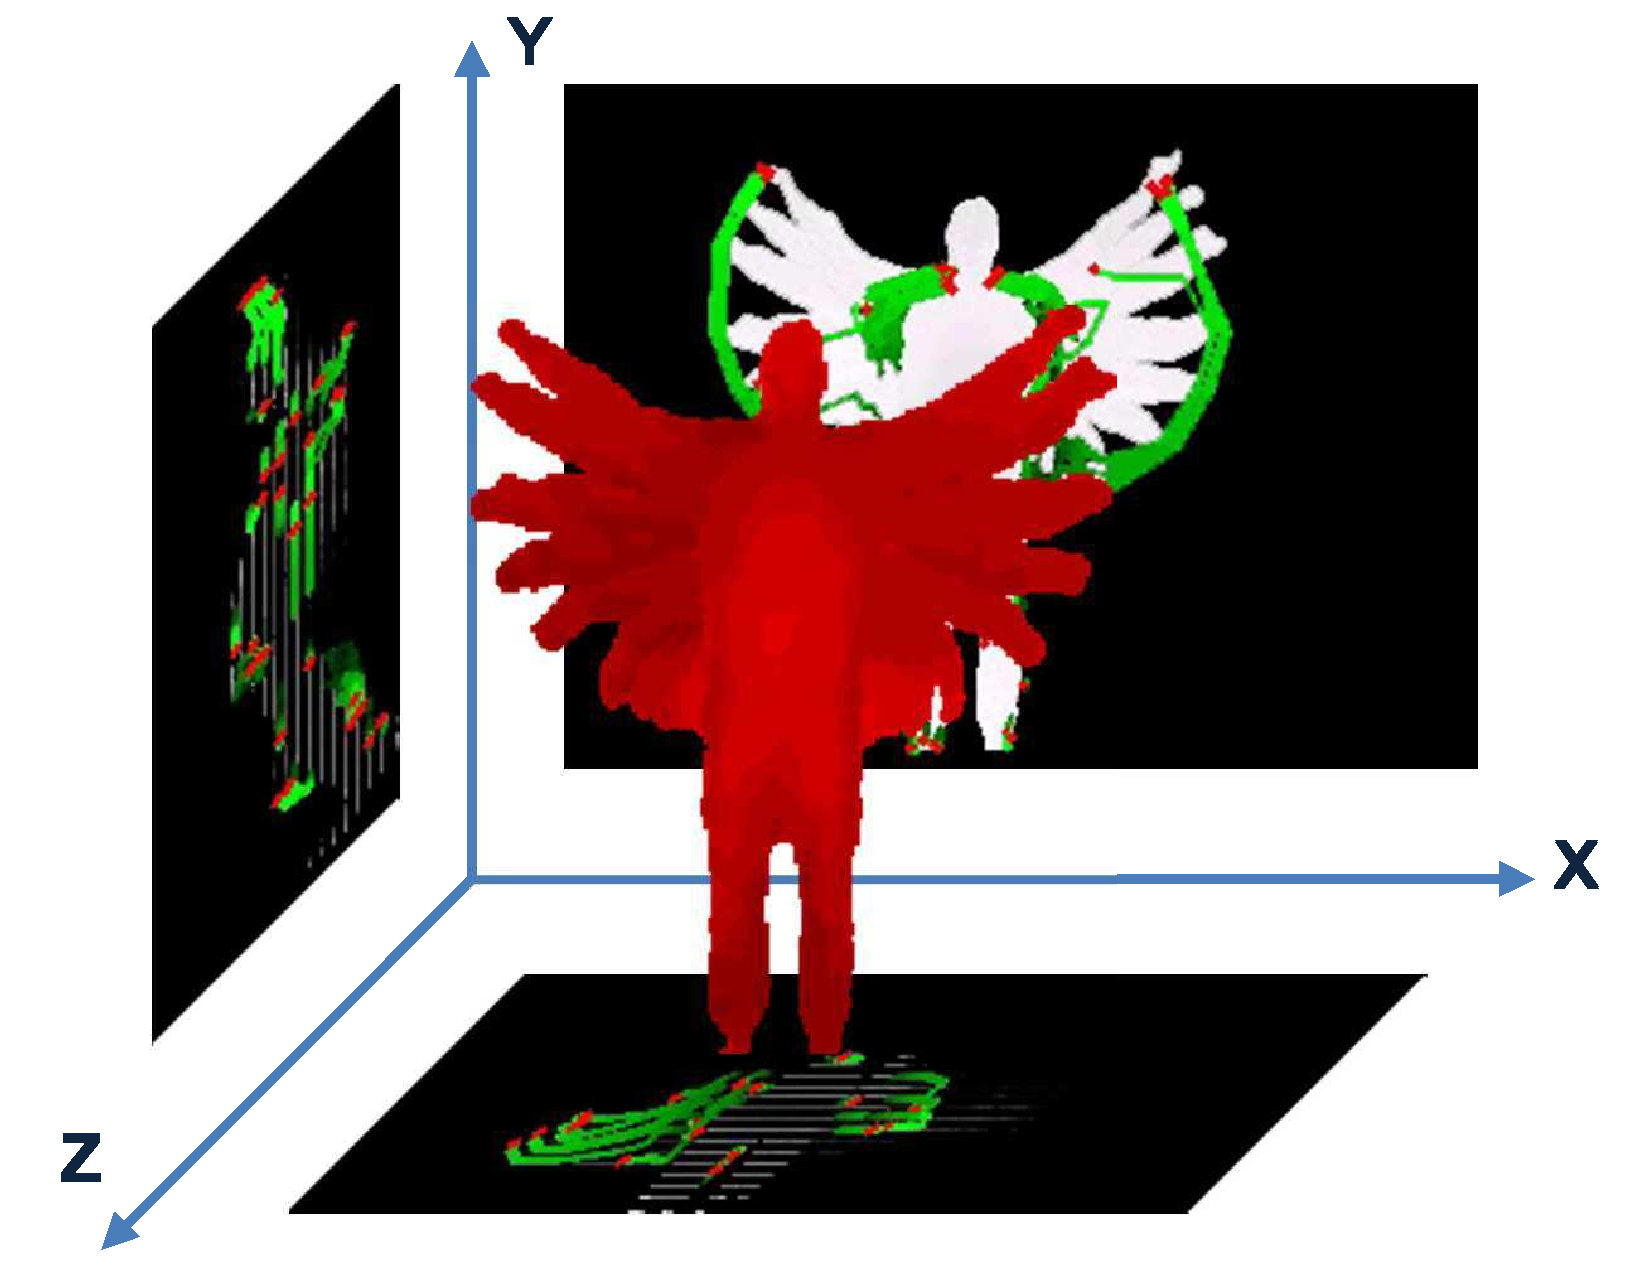
\includegraphics[width=0.47\textwidth]{Projections.pdf}
	\end{center}
	\caption{\label{lbl:Figure_ProposedMethod}Illustration of our trajectory-based approach. The original sequence of depth maps is projected onto three orthogonal planes to form intensity videos. After that, the dense trajectory motion features are calculated for each representation.}
\end{figure}

The basis idea to deal with such cases is to view actions from various directions.
Information achieved from the view directions can provide clearer cues to discriminate such actions.
To collect such information from depth video, a simple way is to project depth maps onto view planes, see figure \ref{lbl:Figure_ProposedMethod}.
The projections are easily obtained by the mentioned advantages of depth data.
Data projected on the planes is then gathered to generate corresponding 2D videos.
Dense trajectory-based motion features are then calculated on 2D videos to generate a final feature representation for depth video.

%\paragraph{Experiments and Results}
To evaluate the effectiveness of our method, we conduct experiments on MSR Action 3D dataset and MSR Daily Activity 3D dataset.
Experimental results show that our proposed method beats the state-of-the-art methods in constrain of only using depth data.
The results also present our contributions: (1) we propose an effective method to exploit trajectories in depth video, (2) we perform comprehensive experiments on the challenging benchmark dataset and indicate that our proposed method is the best when compared with the state-of-the-art depth-based methods.

%\paragraph{Paper structure}
After a brief review of the related work in Section \ref{lbl:RelatedWorks}, the proposed method is described in Section \ref{lbl:ProposedMethod}. Sections \ref{lbl:ExperimentalSettings} and \ref{lbl:ExperimentalResults} present the experimental settings and results. In section \ref{lbl:Discussions} we provide some concerned discussions. The summaries of our work are given in Section \ref{lbl:Conclusions}.

\section{Related Works}
\label{lbl:RelatedWorks}

In terms of action recognition in 2D video, there are three popular approaches used in several action recognition systems, including silhouette-based, salient point-based and trajectory-based.
The silhouette-based approach, as described in \cite{blank2005actions, ke2007event, vitaladevuni2008action, yilmaz2005actions}, is powerful since it encodes a great deal of information in a sequence of images.
However, it is sensitive to different viewpoints, noise and occlusions.
Besides, it depends on the accuracy of localization, background subtraction or tracking for exactly extracting region of interest.
An other approach based on salient points generates a compact video representation and accepts background clutter, occlusions and scale changes.
The effectiveness of this approach is also showed in several works \cite{laptev2005space, dollar2005behavior, laptev2008learning, bregonzio2009recognising, klaser2008aspatiotemporal, willems2008efficient}.
However, in case of recognizing complicated motions, the salient point-based approach deals with several challenges, due to the lack of relationship of salient points.
In recent studies \cite{matikainen2009trajectons, messing2009activity, sun2009hierarchical}, the trajectory-based approach captures moving patterns in video, thereby it provides additional information to recognize motions more exactly.

For depth video, most recent methods exploit depth information into two major directions. The first one is to adapt 2D techniques-based methods for depth data. The second one is to use depth value as its mean.

For the first direction, Yang.X et al. \cite{yang2012recognizing} propose the Depth Motion Maps (DMM) to accumulate global activities in depth video sequences. The DMM are generated by stacking motion energy of depth maps projected onto three orthogonal Cartesian planes. And the Histogram of Oriented Gradients (HOG) \cite{dalal2005histograms} are computed from the DMM to represent an action video. Another approach proposed by Xia.L and Aggarwal.J.K \cite{xia2013spatio} presents a filtering method to extract spatio-temporal interest points from depth videos (DSTIPs). In this approach, they extend a work of Dollar et al. \cite{dollar2005behavior} to adapt for depth data. Firstly, 2D and 1D filters (e.g. Gaussian and Gabor filters) are applied respectively on to the spatial dimensions and temporal dimension in depth video. A correction function then is used to suppress points as depth noises. Finally, points with the largest responses by this filtering method will be selected as the DSTIPs for each video. Besides, a depth cuboid similarity feature (DCSF) is proposed to describe a 3D cuboid around the DSTIPs with supporting size to be adaptable to the depth.

For the second direction, \cite{li2010action} used a bag of 3D points to characterize a set of salient postures. The 3D points are extracted on the contours of the planar projections of the 3D depth map. And then, about 1\% 3D points are sampled to calculate feature. Unlike \cite{li2010action}, \cite{vieira2012stop, wang2012robust, wang2012mining} use occupancy patterns to represent features in action videos.

Vieira et al. \cite{vieira2012stop} proposed a new feature descriptor, called Space-Time Occupancy Patterns (STOP). This descriptor is formed by sparse cells divided by the sequence of depth maps in a 4D space-time grid. The values of the sparse cells are determined by points inside to be on the silhouettes or moving parts of the body. Wang et al. \cite{wang2012robust} presented semi-local features called Random Occupancy Pattern (ROP) features from randomly sampled 4D sub-volumes with different sizes and different locations. The random sampling is performed under a weighted scheme to effectively explore the large dense sampling space. Besides, authors also apply a sparse coding approach to robustly encode these features. The work by Wang et al. \cite{wang2012mining} designed a feature to describe the local ``depth appearance'' for eah joint, named Local Occupancy Patterns (LOP). The LOP features are computed based on 3D point cloud around a particular joint. Moreover, they concatenate the LOP features with skeleton information-based features and apply Short Fourier Transform to obtain the Fourier Temporal Pyramid features at each joint. The Fourier features are utilized in a novel actionlet ensemble model to represent each action video.

Recently, Oreifej and Liu \cite{oreifej2013hon4d} presented a new descriptor for depth maps, named Histogram of Oriented 4D Surface Normals (HON4D). To construct the HON4D, firstly, the 4D normal vectors are computed from the depth sequence. At the next step, the 4D normal vectors is distributed into spatio-temporal cells. To quantize the 4D normal vectors, the 4D space is quantized by using vertices of a regular polychoron. The quantization, then, is refined by additional projectors to make the 4D normal vectors in each cell denser and more discriminative. Afterwards, the HON4D features in cells are concatenated to represent a depth action video.

Inspired by results of Shotton et al. \cite{shotton2013real} and Xia.L et al. \cite{xia2011human}, the work by Yang et al. \cite{yang2012eigenjoints} developed the EigenJoints features based on skeleton information from RGBD sequences. The features contain three feature channels: posture, motion and offset. The posture and motion features represent spatial and temporal information, respectively. The offset features encode the difference between a pose with the initial pose in assumption that the initial pose is neutral. The three channels, then, are normalized and reduced by applying PCA method to obtain the EigenJoints descriptor.

Different from the previous approaches, we use a dense trajectory-based approach for action recognition. We do not care to segment human body like \cite{li2010action,yang2012recognizing}. Besides, skeleton extraction used in \cite{yang2012eigenjoints, wang2012mining} is not also required in our work. We only investigate the benefit of generating 2D transformed videos from depth data, as mentioned in \cite{li2010action,yang2012recognizing}. Moreover, we leverage the effectiveness of trajectory feature to represent an action video. In our best knowledge, no method has previously proposed to adapt the dense trajectory-based approach for human action recognition in depth video. We conduct evaluations on recognition accuracy in depth video using dense trajectories proposed by Wang et al. \cite{wang2011densetraj}.

\section{Proposed Method}
\label{lbl:ProposedMethod}

This paper presents an effective method for action recognition on depth video by adapting the dense trajectory-based motion feature. First, we provide a brief review of the dense trajectory-based feature proposed by Wang.H et al. \cite{wang2011densetraj}. Related parts, such as: dense sampling, tracking and feature descriptors are also referred to. Our dense trajectory-based approach on depth video is mentioned at the end of this section.

\subsection{Dense trajectories}
% - Giới thiệu khái quát về dense trajectories
Trajectories provide a compact representation of motion information in video.
Trajectories from intensity videos can be used for multimedia event detection (MED), video mining, action classification and so on.
Trajectory extraction much depends on both processes: sampling and tracking.
Some concerned methods, such as \cite{matikainen2009trajectons, messing2009activity} used KLT tracker \cite{lucas1981iterative}, or \cite{sun2009hierarchical} matched SIFT descriptors between consecutive frames to obtain feature trajectories.
Recently, the dense trajectory-based motion feature proposed by \cite{wang2011densetraj} has achieved the state-of-the-art performances on MED systems, such as, segment-based system \cite{phan2014multimedia} on TRECVID MED 2010, 2011, or AXES \cite{oneata2012axes}, and BBNVISER \cite{natarajan2012bbn} on TRECVID MED 2012.

In order to obtain trajectories, there are two important steps: sampling and tracking. \cite{wang2011densetraj} propose sampling on a dense grid with a step size of 5 pixels. The sampling is performed at multiple scales with a factor of $1/\sqrt{2}$. Then, tracking is the next step to form trajectories. At each scale, in frame \textit{t}, each point \textit{$P_t = (x_t, y_t)$} is tracked to point \textit{$P_{t+1} = (x_{t+1}, y_{t+1})$} in next frame \textit{t+1} by:
\begin{equation}
	\textit{$P_{t+1} = (x_{t+1}, y_{t+1}) = (x_t, y_t) + (M*\omega)|_{(\bar{x}_t,\bar{y}_t)} $},
\end{equation}
where \textit{$\omega = (u_t, v_t)$} denotes the dense optical flow field, \textit{M} is the kernel of median filtering, and \textit{$(\bar{x}_t,\bar{y}_t)$} is the rounded position of \textit{$P_t$}. The algorithm of \cite{farneback2003two} is adopted to compute the dense optical flow. And to avoid a drifting problem, a suitable value of trajectory length is set to 15 frames. Besides, trajectories with sudden changes are removed.

After extracting trajectories, two kinds of descriptors: a trajectory shape descriptor and a trajectory-aligned descriptor can be adopted. In our experiments, we only use trajectory-aligned descriptors including the HOG \cite{dalal2005histograms}, the Histogram of Optical Flow (HOF) \cite{laptev2008learning}, and the Motion Boundary Histogram (MBH) \cite{dalal2006human}. HOG captures local appearance information, while HOF and MBH encode local motion pattern. The descriptors are computed within a space-time volume ($N \times N$ spatial pixels and $L$ temporal frames) around the trajectory. This volume is divided into a 3D grid (spatially $n_\sigma \times n_\sigma$ grid and temporally $n_\tau$ segments). The default settings of these parameters are $N$ = 32 pixels, $L$ = 15 frames, $n_\sigma$ = 2, and $n_\tau$ = 3.

\iffalse
\paragraph{Trajectory Shape Descriptor}This descriptor describes the shape of a trajectory in the simplest way. Given a trajectory of length L, its shape is concatenated by a sequence of displacement vectors \textit{$S = (\Delta P_t, ..., \Delta P_{t+L-1})$}, where \textit{$\Delta P_t = P_{t+1} - P_t = (x_{t+1} - x_t, y_{t+1} - y_t)$}. In order to make the descriptor invariant to scale changes, the final result is then achieved by normalizing the shape vector by the overall magnitude of the displacement vectors:

\begin{equation}
	\textit{$\bar{S} = \frac{(\Delta P_t, ..., \Delta P_{t+L-1})}{\sum_{k=t}^{t+L-1}\|\Delta P_k\|}$},
\end{equation}
\fi
%\paragraph{Trajectory-aligned Descriptor}
%In order to capture the local motion and appearance around a trajectory, three kinds of descriptors have been employed: the HOG \cite{dalal2005histograms}, the Histogram of Optical Flow (HOF) \cite{laptev2008learning}, and the Motion Boundary Histogram (MBH) \cite{dalal2006human}. For HOG, orientation information is quantized into 8-bin histogram. HOF is 9-bin histogram. Since the feature of a trajectory is calculated and concatenated from sub-volumes of a 3D volume, the final representation has 96 dimensions for HOG and 108 dimensions for HOF. MBH descriptor computes derivatives on both horizontal and vertical components of optical flow $I_\omega = (I_x. I_y)$. Similar to HOG descriptor, the orientation information is quantized into 8-bin histogram. Since the motion information is combined along two directions, the final representation is $96 \times 2 = 192$-bin histogram. By presenting gradient of optical flow, MBH descriptor is able to suppress global motion information and only keep local relative changes in pixels.

According to the authors \cite{laptev2008learning, wang2011densetraj, wang2009evaluation, liu2009recognizing}, all the three descriptors have shown the effectiveness for action recognition. The experimental settings for these descriptors are based on an empirical study showed in \cite{wang2011densetraj}. We also conduct our experiment on all the three descriptors when compared to the depth-based state-of-the-art methods.

\subsection{Proposed Method for Dense Trajectory-based Approach}

Our proposed method to adapt the dense trajectory-based approach for human action recognition in depth video is as follow. At first, intensity videos are formed from the sequence of depth maps, as illustrated in figure \ref{lbl:Figure_ProposedMethod}. At this step, to obtain an intensity video from a view direction $\alpha$, corresponding to a view plane $\mathcal{P}(\alpha): ax + by + cx + d = 0$, in each depth map $t$, each point $P_t(x_t,y_t,z_t)$ is projected to $P_\mathcal{P}(x_\mathcal{P},y_\mathcal{P},z_\mathcal{P})$ on the view plane $\mathcal{P}(\alpha)$, see in figure \ref{lbl:Figure_PointProjection}, by:

\begin{figure}
	\centering
	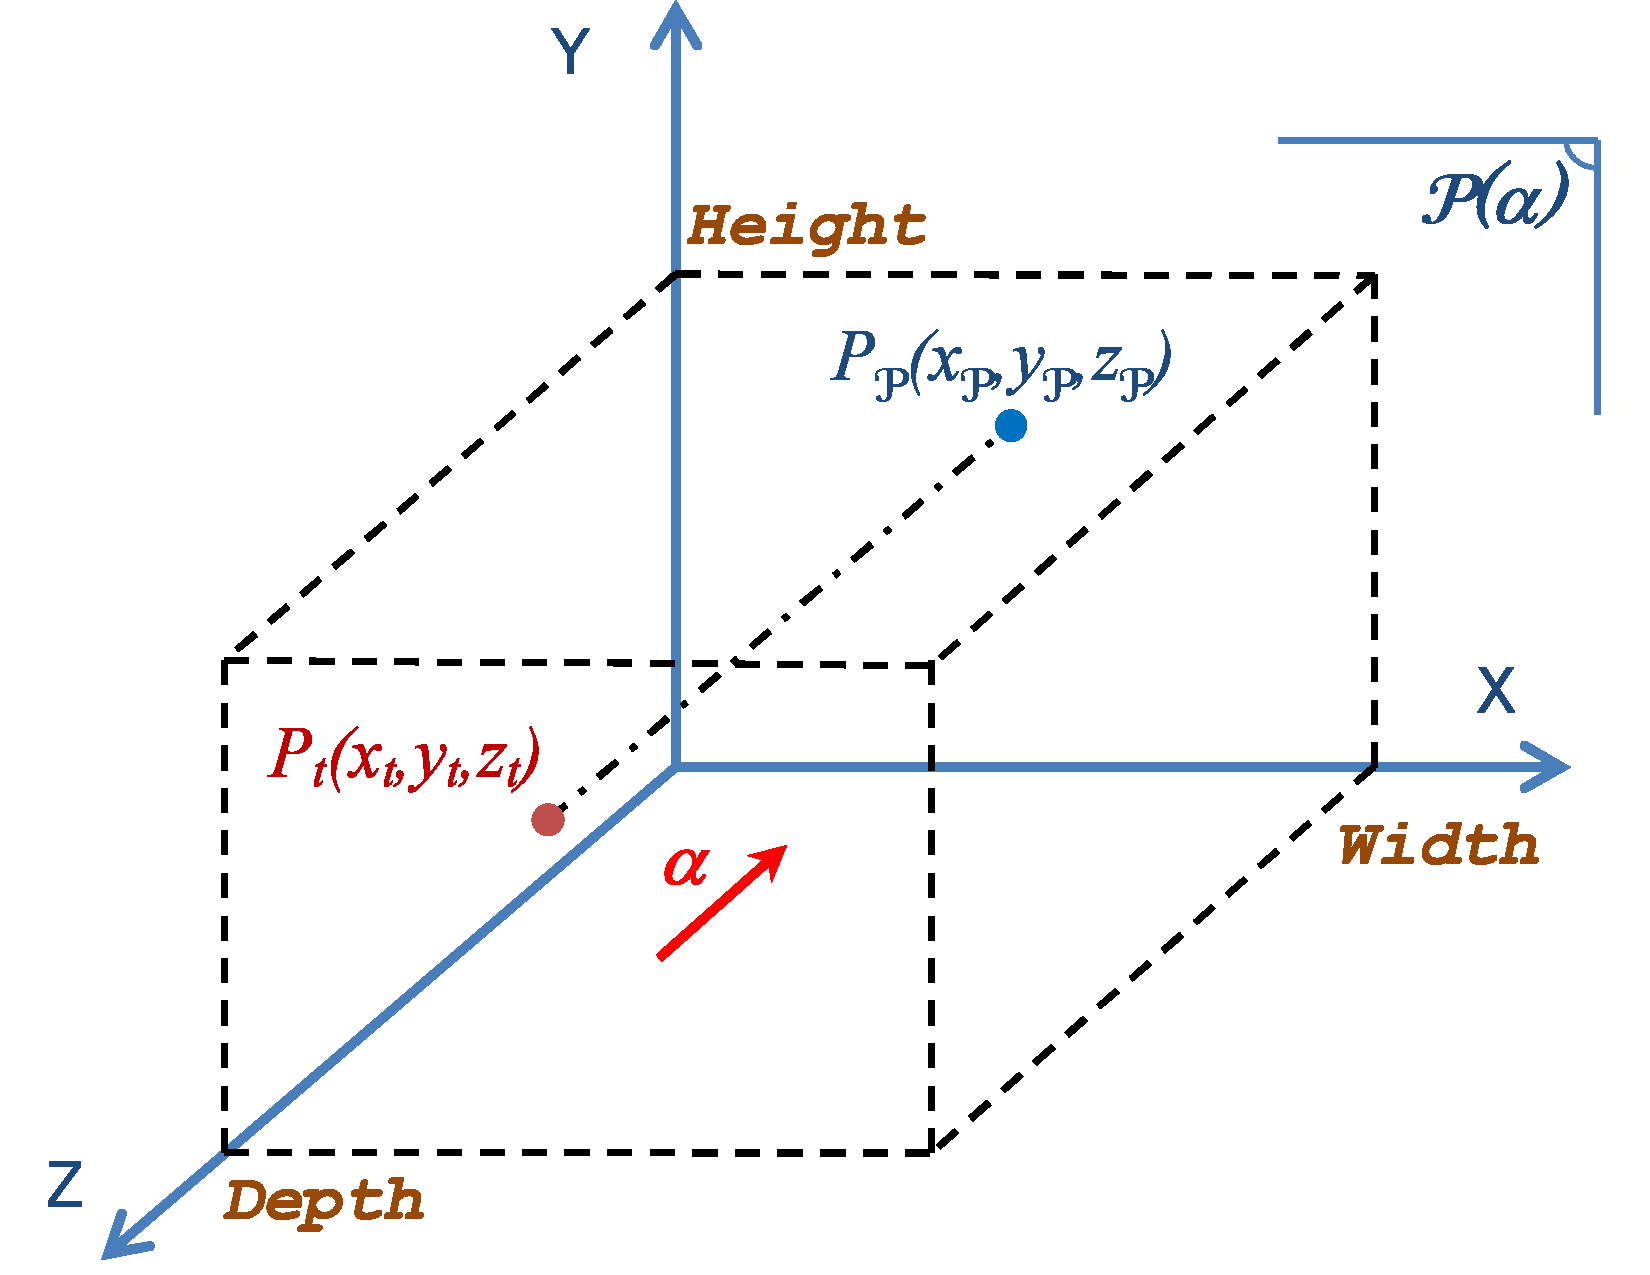
\includegraphics[width=0.47\textwidth]{Figure_PointProjection.pdf} %
	\caption{\label{lbl:Figure_PointProjection}An illustration of the projection. Point $P_\mathcal{P}$ is the projection of point $P_t$ along a view direction $\alpha$ onto a view plane $\mathcal{P}(\alpha)$.}
\end{figure}

\begin{equation}
	P_t(x_t,y_t,z_t)\xrightarrow{\mathcal{P}(\alpha)}P_\mathcal{P}(x_\mathcal{P},y_\mathcal{P},z_\mathcal{P})
\end{equation}

where,
\begin{equation}
	x_\mathcal{P} = x_t - \frac{ax_t + by_t + cz_t + d}{a^2 + b^2 + c^2}a
\end{equation}
\begin{equation}
	y_\mathcal{P} = y_t - \frac{ax_t + by_t + cz_t + d}{a^2 + b^2 + c^2}b
\end{equation}
\begin{equation}
	z_\mathcal{P} = z_t - \frac{ax_t + by_t + cz_t + d}{a^2 + b^2 + c^2}c
\end{equation}
And the intensity value $v$ at the projected point $P_\mathcal{P}$ is computed by:
\begin{equation}
	v(P_\mathcal{P}) = \frac{ax_t + by_t + cz_t + d}{\sqrt{a^2 + b^2 + c^2}}
\end{equation}
So, given a set of 3D points $\mathcal{S}(t) = \{(x_t,y_t,z_t)\vert(x_t,y_t,z_t) \in t\}$, we have a projection $\mathcal{S}_\alpha(t) = \{(x_\mathcal{P},y_\mathcal{P},z_\mathcal{P})\vert(x_\mathcal{P},y_\mathcal{P},z_\mathcal{P}) \in \mathcal{P}(\alpha)\}$. Therefore, a set of the projections obtained from a given sequence of M depth maps under a view direction $\alpha$ is an expected intensity video $\mathcal{R}(\alpha) = \{\mathcal{S}_\alpha(t) \vert t=\overline{1..M}\}$. Each intensity video obtained from the corresponding projection onto the sequence of depth maps can be regarded as a 2D transformed video of action in depth video.

In particular, we choose three representations to represents for three view directions: front, side, and top in 3D space, corresponding to three view planes, respectively: $Oxy$, $Oyz$ and $Ozx$. With these view directions, the corresponding projections are respectively:
\begin{equation}
\mathcal{S}_\text{front}(t) = \{(x_t,y_t,0)\vert(x_t,y_t,0) \in \mathcal{P}:z=0\}
\end{equation}
\begin{equation}
\mathcal{S}_\text{side}(t) = \{(0,y_t,z_t)\vert(0,y_t,z_t) \in \mathcal{P}:x=0\}
\end{equation}
\begin{equation}
\mathcal{S}_\text{top}(t) = \{(x_t,0,z_t)\vert(x_t,0,z_t) \in \mathcal{P}:y=0\}
\end{equation}
And the corresponding intensity values in the three projections are, respectively:
\begin{equation}
	v(P_\text{front}) = z_t
\end{equation}
\begin{equation}
	v(P_\text{side}) = x_t
\end{equation}
\begin{equation}
	v(P_\text{top}) = y_t
\end{equation}

\subsection{Our framework overview}

In this section, we provide a brief introduction about our framework for action recognition task.
The first step is to transform projection results from sequences of depth maps into corresponding 2D videos.
Transforming depth video into the 2D videos is necessary due to dimensional gap when we adapt 2D techniques for 3D data.
Afterwards, the dense trajectories \cite{wang2011densetraj} are extracted from the 2D transformed videos.
With this approach, we do not care the challenges from human body segmentation as well as skeleton extraction.
Trajectory-aligned descriptors are computed then. At the next step, with each 2D transformed video $\mathcal{R}(\alpha_i)$, $i = \overline{1..N}$, corresponding feature representation $F(\alpha_i) = (b^1_\text{$\alpha_i$},b^2_\text{$\alpha_i$},...,b^K_\text{$\alpha_i$})$ is quantized from a set of raw trajectory features using a bag-of-words (BoW) model with $K$ visual words.
For quantization, the hard-assignment technique is used to compute histograms of the visual words on the 2D transformed videos.
An \textit{early fusion} scheme which integrates unimodal features before learning, then, is used to generate feature representation $\mathcal{F} = (F(\alpha_1),...,F(\alpha_N))$ for action in the sequence of depth maps.
After the final feature representations are generated, we adopt the popular Support Vector Machine (SVM) for classification. In practice, we use the precomputed-kernel technique with the histogram intersection kernel for the classification step.
Besides, we perform the one-vs-all strategy for multi-class classification.

\begin{figure*}[t]
	\centering
		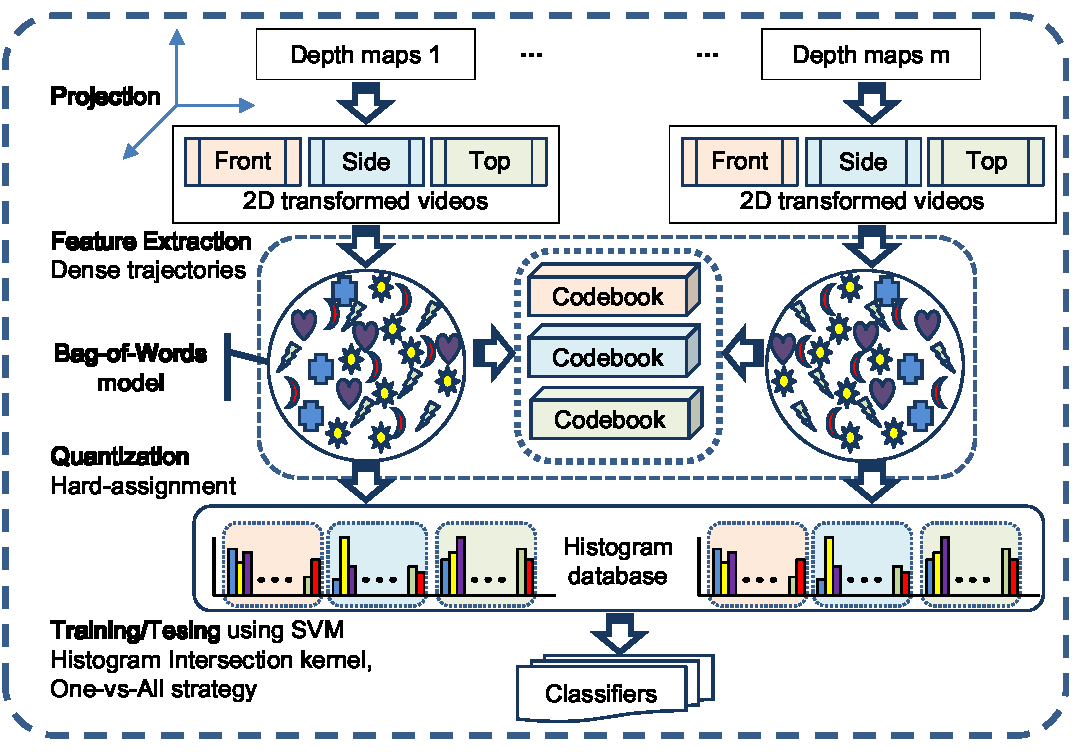
\includegraphics[width=0.9\textwidth]{Framework3D.pdf} %
	\caption{\label{lbl:Figure_Framework}Our Framework Overview}
\end{figure*}
%- Hình 3 - Framework overview for our system - Depth data -> 3 feature extraction -> 3 BoW model -> 3 histogramintersection-SVM -> concatenated-score features -> chi-kernel SVM classifier

%In order to generate intensity representations from the sequence of depth maps, we use the approach proposed in \cite{li2010action}. This technique is also used in \cite{yang2012recognizing}. Basically, this method projects depth maps onto three orthogonal planes in Casterian space to obtain corresponding intensity representations. However, motion representation for human action in the previous approaches is accumulated from global motion information. Therefore, these approaches must deal with the challenges from human segmentation problem in more complicated datasets. In contrast to the previous ones, we pay attention to capture local motion information for representing human actions. With the approach, we do not care the challenges for segmenting human body. To effectively use local motion information, we leverage the effectiveness of trajectory-based representation. In practice, we adopt the dense trajectory-based approach proposed in \cite{wang2011densetraj}. Thus, motion information in depth data can be reproduced by complementary motion information from different intensity representations.

Our proposed trajectory-based approach is compared with the state-of-the-art methods in human action recognition using depth data. Actually, our approach does not care skeleton extraction, which is used as an important factor in some works, such as \cite{wang2012mining, yang2012eigenjoints}. In fact, extracting skeleton exactly is still an completely unsolved problem, due to the challenges, such as cluttered background, hardware quality, camera motion, so on.

\section{Experimental Settings}
\label{lbl:ExperimentalSettings}

\subsection{Dataset}
\label{lbl:ExperimentalSettings_Dataset}
We test our method on MSR Action 3D dataset. This dataset contains 20 actions, as showed in Table \ref{lbl:20actions}. Actions are performed by ten subjects for two or three times in the context of game console interaction. In total, there are 567 sequences of depth maps. The depth maps are shot at frame rate of 15 fps. The size of the depth map is $640 \times 480$, we resize into $320 \times 240$ to ensure processing efficiency.

\begin{table}[H]
	\begin{center}
		\resizebox{0.47\textwidth}{!}{%
		% Table generated by Excel2LaTeX from sheet 'MSRAction3D names'
		\begin{tabular}{c|c|c|c}
		
		  {\bf   ID  } & {\bf Action Name} &   {\bf   ID  } & {\bf Action Name} \\
		\hline
		             1 &  high arm wave &             11 &  two hand wave \\
		
		             2 & horizontal arm wave &             12 &    side-boxing \\
		
		             3 &         hammer &             13 &           bend \\
		
		             4 &     hand catch &             14 &   forward kick \\
		
		             5 &  forward punch &             15 &      side kick \\
		
		             6 &     high throw &             16 &        jogging \\
		
		             7 &         draw x &             17 &   tennis swing \\
		
		             8 &      draw tick &             18 &   tennis serve \\
		
		             9 &    draw circle &             19 &     golf swing \\
		
		            10 &      hand clap &             20 & pick up \& throw \\
		
		\end{tabular} %
		}
	\end{center}
	\caption{\label{lbl:20actions}20 actions in MSR Action 3D dataset}
\end{table}

In order to conduct a fair comparison, we use the same experimental settings as \cite{li2010action, yang2012eigenjoints, yang2012recognizing, wang2012mining, xia2013spatio, oreifej2013hon4d}. In the settings, the dataset is divided into three action subsets. Each subset has 8 actions (Table \ref{lbl:3ActionSubsets}). The two subsets AS1 and AS2 present that grouped actions have similar movements. The subset AS3 groups complex actions together. For instance, action \textit{hammer} seems to be confused with action \textit{forward punch} in AS1 or similar movements between action \textit{hand catch} and action \textit{side boxing} in AS2. As for each subset, we select half of the subjects as training and the rest as testing (i.e. cross subject test).

\begin{table}[h]
	\begin{center}
		\resizebox{0.47\textwidth}{!}{%
		% Table generated by Excel2LaTeX from sheet 'Sheet3'
		\begin{tabular}{c|c|c}
		
		{\bf Action Subset 1} & {\bf Action Subset 2} & {\bf Action Subset 3} \\
		{\bf(AS1)} & {\bf(AS2)} & {\bf(AS3)} \\
		\hline
		horizontal arm wave &  high arm wave &     high throw \\
		
		        hammer &     hand catch &   forward kick \\
		
		 forward punch &         draw x &      side kick \\
		
		    high throw &      draw tick &        jogging \\
		
		     hand clap &    draw circle &   tennis swing \\
		
		          bend &  two hand wave &   tennis serve \\
		
		  tennis serve &    side-boxing &     golf swing \\
		
		pick up \& throw &   forward kick & pick up \& throw \\
		
		\end{tabular} %
		}
	\end{center}
	\caption{\label{lbl:3ActionSubsets}The three action subsets used in the experiments}
\end{table}

\subsection{Evaluation Framework}

Figure \ref{lbl:Figure_Framework} shows our evaluation framework for the trajectory-based features. We perform experiments using the proposed approach and compare with the state-of-the-art methods on depth data. We use the application available online\footnote{http://lear.inrialpes.fr/$\sim$wang/dense\_trajectories} to extract dense trajectories and aligned-descriptors. Experimental results reported in section \ref{lbl:ExperimentalResults} attach to the MBH descriptor. The HOG, HOF descriptors will be mentioned in the section \ref{lbl:Discussions}. To quantize a large number of features obtained by densely sampling, the BoW model is applied. At first, in each intensity representation, we randomly get about 80,000 extracted trajectories for clustering with K-mean algorithm. Then, a codebook of 2000 visual codewords is formed for each.

In order to classify actions, in our implementation, we use the libSVM library published online by author\footnote{http://www.csie.ntu.edu.tw/$\sim$cjlin/libsvm/}. We adopt the format requirements of the library to synchronize the annotation and the data. For testing, predicted value of each action is defined as the maximum score obtained from all the classifiers. This score shows that a human action is confused with another or not.

\section{Experimental Results}
\label{lbl:ExperimentalResults}
This section presents the experimental results for applying our proposed approach on MSR Action 3D dataset. All experimental results are reported under the settings mentioned in section \ref{lbl:ExperimentalSettings_Dataset}. Besides, in comparison with the state-of-the-art methods, our reported result is calculated on front representation only. In addition, an evaluation related to selecting compensation information from other representations will be also mentioned. All the results are compared in terms of recognition accuracy. The best performance is highlighted in bold.

\subsection{Recognize Actions from An Intensity Representation}

Table \ref{lbl:Table_MBHvsSoAonFront} shows evaluation results of our trajectory-based approach and the state-of-the-art methods in terms of average accuracy  on three action subsets of MSR Action 3D dataset (Table \ref{lbl:3ActionSubsets}). The compared methods are based on various feature representations, such as silhouette features \cite{li2010action, yang2012recognizing}, skeletal joint features like \cite{yang2012eigenjoints, wang2012mining}, local occupancy patterns \cite{wang2012robust, vieira2012stop}, normal orientation features \cite{oreifej2013hon4d} and cuboid similarity features \cite{xia2013spatio}. Interestingly, under the same setting (i.e cross subject test), the result table indicates that our approach beats all of them. Besides, the results also show that there is significant difference of the performance between our method and the rest.

\begin{table}[h]
	\begin{center}
		\resizebox{0.2\textwidth}{!}{%
		% Table generated by Excel2LaTeX from sheet 'VIEWS_LateFusion'
		\begin{tabular}{ccc}
		
		       \multicolumn{ 3}{c}{{\bf Action Subsets}} \\
		\hline
		     {\bf AS1} &      {\bf AS2} &      {\bf AS3} \\
		\hline
		        92.45  &         92.04  &         99.11  \\
		
		\end{tabular} %
		}
	\end{center}
	\caption{\label{lbl:MBHandAS123}Accuracy of our method on three action subsets.}
\end{table}

\begin{table}[h]
	\begin{center}
		\resizebox{0.47\textwidth}{!}{%
		% Table generated by Excel2LaTeX from sheet 'Methods'
		\begin{tabular}{c|c}
		
		  {\bf Method} & {\bf Accuracy (\%)} \\
		\hline
		Bag of 3D Points \cite{li2010action} &         74.70  \\
		
		      STOP \cite{vieira2012stop} &         84.80  \\
		
		EigenJoints \cite{yang2012eigenjoints} &         82.33  \\
		
		Random Occupancy Patterns \cite{wang2012robust} &         86.50  \\
		
		Local Occupancy Patterns \cite{wang2012mining} &         88.20  \\
		
		Depth Motion Maps-based HOG \cite{yang2012recognizing} &         91.63  \\
		
		Histogram of Oriented 4D Normals \cite{oreifej2013hon4d} &         88.89  \\
		
		Depth Cuboid Similarity Feature \cite{xia2013spatio} &         89.30  \\
		\hline
		    {\bf Ours} &   {\bf 94.53 } \\
		
		\end{tabular}%
		}
	\end{center}
	\caption{\label{lbl:Table_MBHvsSoAonFront}Comparison of accuracy on MSR Action 3D dataset. Notice that experimental results reported in this table is based on front representation only. Besides, we also use MBH descriptor only to calculate trajectory features.}
\end{table}

Consider the accuracy results on action subsets reported in Table \ref{lbl:MBHandAS123}, we found that two subsets AS1, AS2 contain many confused actions. Considering confusion matrices as showed in Table \ref{lbl:AS123ConfusionMatrix}, some action-pairs are confused, such as: \textit{hammer} (a03) and \textit{forward punch} (a05) in AS1, or \textit{side-boxing} (a12) and \textit{hand catch} (a04) in AS2. When analyzing the confused actions, we found that the main cause is due to similar motions of actions in the same view direction (i.e front representation). Besides, since depth data is textureless, it makes recognizing more difficult. That is reason why we need compensate information from other intensity representations.

\begin{table}[h]
	\begin{center}
		\subfloat[Action Subset 1 \label{lbl:ConfMatAS1}]{ %
		\resizebox{0.8\textwidth}{!}{ %
			% Table generated by Excel2LaTeX from sheet 'Experiment-MSRDaily3D'
			\begin{tabularx}{\textwidth}{c|c|c|c|c|c|c|c|c|}
					\multicolumn{1}{c}{~}& \multicolumn{1}{c}{\bf a02} & \multicolumn{1}{c}{\bf a03} & \multicolumn{1}{c}{\bf a05} & \multicolumn{1}{c}{\bf a06} & \multicolumn{1}{c}{\bf a10} & \multicolumn{1}{c}{\bf a13} & \multicolumn{1}{c}{\bf a18} & \multicolumn{1}{c}{\bf a20} \\
				\hhline{~--------}
					{\bf a02} & \color{white}{\bf 0.83}\cellcolor[gray]{.2} & 0 & {\bf 0.17}\cellcolor[gray]{.8} & 0 & 0 & 0 & 0 & 0 \\
				\hhline{~--------}
					{\bf a03} & 0 & \color{white}{\bf 0.92}\cellcolor[gray]{.1} & {\bf 0.08}\cellcolor[gray]{.9} & 0 & 0 & 0 & 0 & 0 \\
				\hhline{~--------}
					{\bf a05} & 0 & {\bf 0.36}\cellcolor[gray]{.6} & \color{white}{\bf 0.64}\cellcolor[gray]{.4} & 0 & 0 & 0 & 0 & 0 \\
				\hhline{~--------}
					{\bf a06} & 0 & 0 & 0 & \color{white}{\bf 1.0}\cellcolor[gray]{.0} & 0 & 0 & 0 & 0 \\
				\hhline{~--------}
					{\bf a10} & 0 & 0 & 0 & 0 & \color{white}{\bf 1.0}\cellcolor[gray]{.0} & 0 & 0 & 0 \\
				\hhline{~--------}
					{\bf a13} & 0 & 0 & 0 & 0 & 0 & \color{white}{\bf 1.0}\cellcolor[gray]{.0} & 0 & 0 \\
				\hhline{~--------}
					{\bf a18} & 0 & 0 & 0 & 0 & 0 & 0 & \color{white}{\bf 1.0}\cellcolor[gray]{.0} & 0 \\
				\hhline{~--------}
					{\bf a20} & 0 & 0 & 0 & 0 & 0 & {\bf 0.07}\cellcolor[gray]{.9} & 0 & \color{white}{\bf 0.93}\cellcolor[gray]{.1} \\
				\hhline{~--------}
			\end{tabularx} %
		}
		}
		
		\subfloat[Action Subset 2 \label{lbl:ConfMatAS2}]{
		\resizebox{0.8\textwidth}{!}{ %
			% Table generated by Excel2LaTeX from sheet 'Experiment-MSRDaily3D'
			\begin{tabularx}{\textwidth}{c|c|c|c|c|c|c|c|c|}
					\multicolumn{1}{c}{~}& \multicolumn{1}{c}{\bf a01} & \multicolumn{1}{c}{\bf a04} & \multicolumn{1}{c}{\bf a07} & \multicolumn{1}{c}{\bf a08} & \multicolumn{1}{c}{\bf a09} & \multicolumn{1}{c}{\bf a11} & \multicolumn{1}{c}{\bf a12} & \multicolumn{1}{c}{\bf a14} \\
				\hhline{~--------}
					{\bf a01} & \color{white}{\bf 1.0}\cellcolor[gray]{.2} & 0 & 0 & 0 & 0 & 0 & 0 & 0 \\
				\hhline{~--------}
					{\bf a04} & {\bf 0.08}\cellcolor[gray]{.9} & \color{white}{\bf 0.84}\cellcolor[gray]{.2} & {\bf 0.08}\cellcolor[gray]{.9} & 0 & 0 & 0 & 0 & 0 \\
				\hhline{~--------}
					{\bf a07} & 0 & 0 & \color{white}{\bf 0.79}\cellcolor[gray]{.2} & {\bf 0.07}\cellcolor[gray]{.9} & {\bf 0.07}\cellcolor[gray]{.9} & 0 & {\bf 0.07}\cellcolor[gray]{.9} & 0 \\
				\hhline{~--------}
					{\bf a08} & 0 & 0 & 0 & \color{white}{\bf 1.0}\cellcolor[gray]{.0} & 0 & 0 & 0 & 0 \\
				\hhline{~--------}
					{\bf a09} & 0 & 0 & 0 & {\bf 0.13}\cellcolor[gray]{.9} & \color{white}{\bf 0.87}\cellcolor[gray]{.1} & 0 & 0 & 0 \\
				\hhline{~--------}
					{\bf a11} & 0 & 0 & 0 & 0 & 0 & \color{white}{\bf 1.0}\cellcolor[gray]{.0} & 0 & 0 \\
				\hhline{~--------}
					{\bf a12} & 0 & {\bf 0.13}\cellcolor[gray]{.9} & 0 & 0 & 0 & 0 & \color{white}{\bf 0.87}\cellcolor[gray]{.1} & 0 \\
				\hhline{~--------}
					{\bf a14} & 0 & 0 & 0 & 0 & 0 & 0 & 0 & \color{white}{\bf 1.0}\cellcolor[gray]{.0} \\
				\hhline{~--------}
			\end{tabularx} %
		}
		}
		
		\subfloat[Action Subset 3 \label{lbl:ConfMatAS3}]{
		\resizebox{0.8\textwidth}{!}{ %
			% Table generated by Excel2LaTeX from sheet 'Experiment-MSRDaily3D'
			\begin{tabularx}{\textwidth}{c|c|c|c|c|c|c|c|c|}
					\multicolumn{1}{c}{~}& \multicolumn{1}{c}{\bf a06} & \multicolumn{1}{c}{\bf a14} & \multicolumn{1}{c}{\bf a15} & \multicolumn{1}{c}{\bf a16} & \multicolumn{1}{c}{\bf a17} & \multicolumn{1}{c}{\bf a18} & \multicolumn{1}{c}{\bf a19} & \multicolumn{1}{c}{\bf a20} \\
				\hhline{~--------}
					{\bf a06} & \color{white}{\bf 1.0}\cellcolor[gray]{.0} & 0 & 0 & 0 & 0 & 0 & 0 & 0 \\
				\hhline{~--------}
					{\bf a14} & 0 & \color{white}{\bf 1.0}\cellcolor[gray]{.0} & 0 & 0 & 0 & 0 & 0 & 0 \\
				\hhline{~--------}
					{\bf a15} & 0 & 0 & \color{white}{\bf 1.0}\cellcolor[gray]{.0} & 0 & 0 & 0 & 0 & 0 \\
				\hhline{~--------}
					{\bf a16} & 0 & 0 & 0 & \color{white}{\bf 1.0}\cellcolor[gray]{.0} & 0 & 0 & 0 & 0 \\
				\hhline{~--------}
					{\bf a17} & 0 & 0 & 0 & 0 & \color{white}{\bf 1.0}\cellcolor[gray]{.0} & 0 & 0 & 0 \\
				\hhline{~--------}
					{\bf a18} & 0 & 0 & 0 & 0 & 0 & \color{white}{\bf 0.93}\cellcolor[gray]{.1} & {\bf 0.07}\cellcolor[gray]{.9} & 0 \\
				\hhline{~--------}
					{\bf a19} & 0 & 0 & 0 & 0 & 0 & 0 & \color{white}{\bf 1.0}\cellcolor[gray]{.0} & 0 \\
				\hhline{~--------}
					{\bf a20} & 0 & 0 & 0 & 0 & 0 & 0 & 0 & \color{white}{\bf 1.0}\cellcolor[gray]{.0} \\
				\hhline{~--------}
			\end{tabularx} %
		}
		}
		
	\end{center}
	\caption{\label{lbl:AS123ConfusionMatrix}Confusion matrices on three action subsets. Notice that action names are identified by indices of actions in table \ref{lbl:20actions}}
\end{table}

\subsection{Compensate Motion Information from Other Representations}
In this part, we conduct experiments based on compensating information from other representations (i.e side and top) for the front representation. We report the experimental results on three action subsets and the average of the three subsets. Figure \ref{lbl:Figure_EarlyFusion_AS123_MBH} shows a better view in comparing the fusion of front, side and top representations with the separate representations. Expectedly, the average recognition accuracy of the fusion, which is 96.67\% accuracy, is better than the average recognition accuracy of the representations on the average of the three action subsets. Obviously, our proposed approach outperforms the mentioned state-of-the-art methods.
 
Besides, based on experimental results in figure \ref{lbl:Figure_EarlyFusion_AS123_MBH}, compensating information indicates two interesting points. The first one confirms that recognition result from front representation is better than the others (i.e. side and top). The second one shows that compensated information from other representations for front representation supports final predictions effectively. Thus, our proposed approach can be applied for any intensity-based techniques, in general.

\begin{figure}[h]
	\begin{center}
		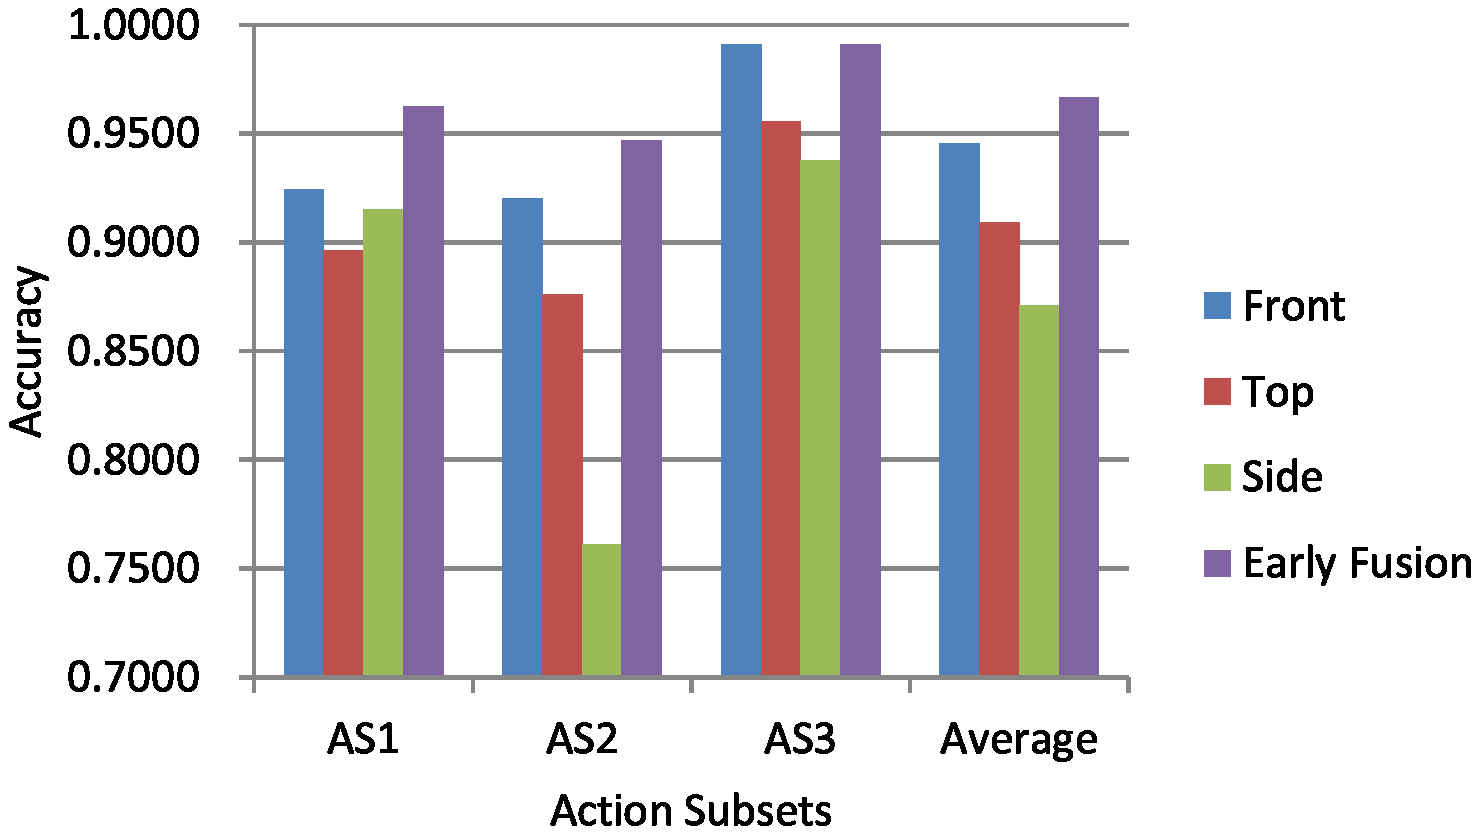
\includegraphics[width=0.47\textwidth]{Chart_EarlyFusion_AS123_MBH.eps}
	\end{center}
	\caption{\label{lbl:Figure_EarlyFusion_AS123_MBH}Comparison of recognition accuracy by using the early fusion scheme on intensity representations.}
\end{figure}

\section{Discussions}
\label{lbl:Discussions}

\subsection{The Impact of Our Method on Descriptors}

For intensity data, according to \cite{wang2011densetraj} MBH is the best feature descriptor for dense trajectories. Therefore, in previous experiments, we only use MBH descriptor to represent motion information. Due to the difference between depth data and intensity data, how our approach has influenced other trajectory-aligned descriptors (i.e. HOG, HOF). In this section, we conduct similar experiments on these descriptors to answer this issue.

\begin{figure}[h]
	\begin{center}
		\includegraphics[width=0.47\textwidth]{Chart_ImpactOfDescriptors.eps}
	\end{center}
	\caption{\label{lbl:Figure_MBHHOGHOF}Comparison of recognition accuracy on trajectory-aligned descriptors.}
\end{figure}

In this part, we report the average recognition accuracies on the three descriptors and on the separate representations (i.e. front, side and top) as well as the fusion of the three representations. Figure \ref{lbl:Figure_MBHHOGHOF} shows interesting results. Although, recognition results on descriptors HOG, HOF are not good for each intensity representation, the final results after fusing have been significantly improved. The results indicate that the performances of HOG and HOF, respectively 94.53\% and 92.42\%, also outperform the state-of-the-art methods, as mentioned in table \ref{lbl:Table_MBHvsSoAonFront}. In addition, lower-cost descriptors like HOG, HOF have more benefits for decreasing computational cost in processes, such as feature extraction and video representation (using the BoW model). These advantages provide a promising way for building effective and efficient systems.

\subsection{Evaluate the Role of Intensity Representations}

In this section, we consider the role of representations to our proposed method. Figure \ref{lbl:Figure_EarlyFusion_AS123_MBH} confirms that front representation achieves the best result. Obviously, it is an indispensable component to merge information. For the rest, we perform experiments on representation combinations with front representation. Experimental results are reported in figure \ref{lbl:Figure_CombinationsFRONTSIDETOP}. In this experiment, the recognition accuracies of combinations are calculated on each intensity representations and the fusion.

\begin{figure}[h]
	\begin{center}
		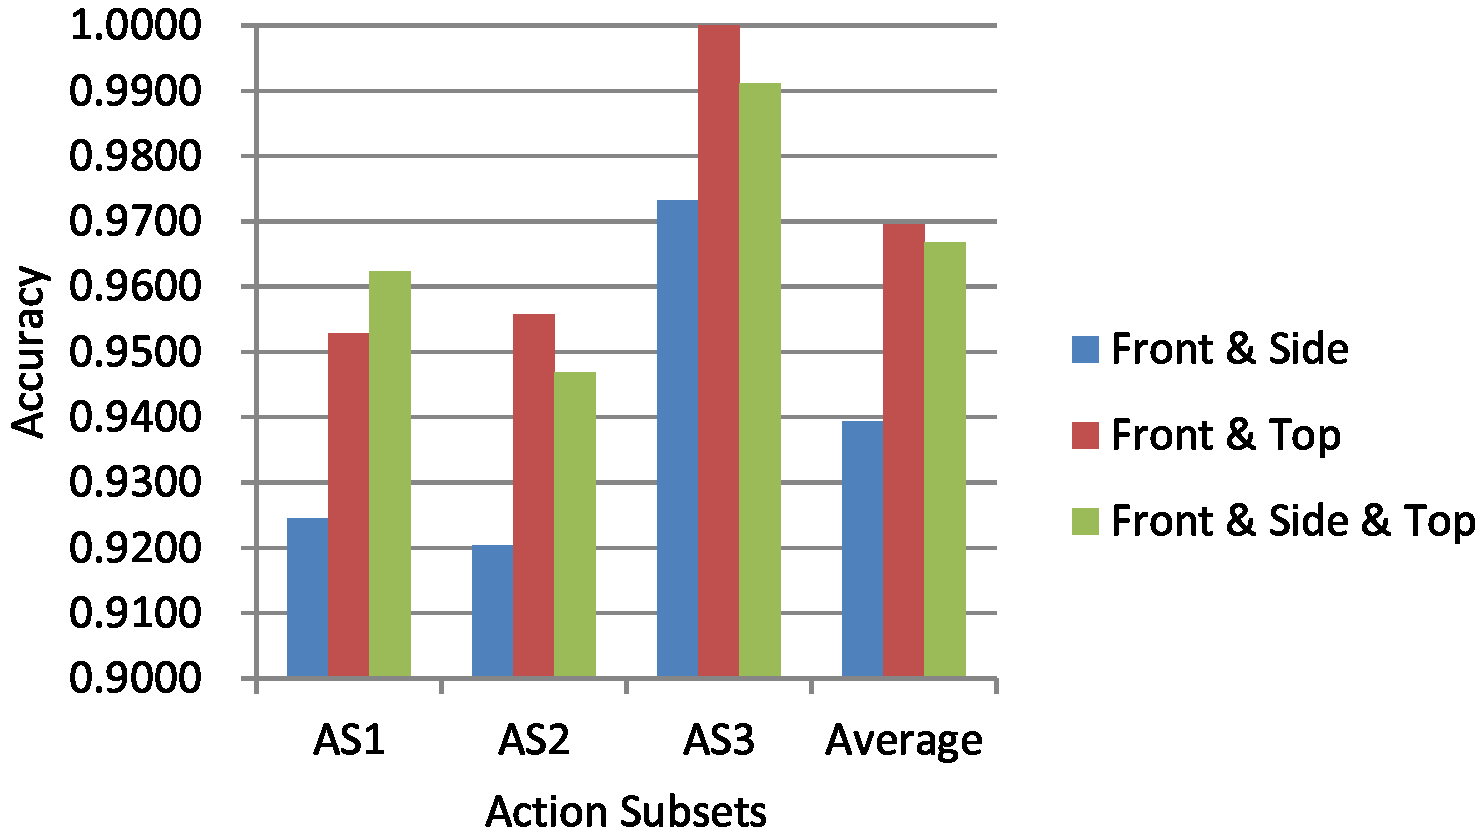
\includegraphics[width=0.47\textwidth]{Chart_RoleOfRepresentations.eps}
	\end{center}
	\caption{\label{lbl:Figure_CombinationsFRONTSIDETOP}Comparison of recognition accuracy on combinations of intensity representations.}
\end{figure}

In order to conduct the experiments, we create combinations: front and side, front and top. Figure \ref{lbl:Figure_CombinationsFRONTSIDETOP} indicates that the combination of front and top is better than the combination of front and side. More interestingly, the achieved performance, which is 96.95\% accuracy, from the combination of front and top beats the performance based on combining all the representations, in terms of average. Actually, the discovery provides a good choice to decrease computational cost but still ensures a convincing performance.

\subsection{MSR Daily Activity 3D Dataset}

 The  MSR Daily Activity 3D dataset is proposed by \cite{wang2012mining}, which includes 16 daily activities  (Fig. \ref{lbl:Figure_MSRDaily3D}) such as talking on the phone, reading a book, playing game, ... etc. In this dataset, background objects and subjects appear at different distances to the camera. Table \ref{lbl:Table_Daily3D} shows a comparison of recognition accuracies between the state-of-the-art methods on MSR Daily Activity 3D dataset. In this experiment, we conduct our trajectory-based approach only on front representation and use MBH descriptor to describe motion feature. In addition, we follow the experimental settings as described in \cite{wang2012mining}. In condition of only using depth data, \cite{wang2012mining, oreifej2013hon4d, xia2013spatio} report a unexpected performance. In \cite{xia2013spatio}, they modified this dataset to do evaluation. It is not fair to compare. Therefore, to ensure a fair comparison, we follow a framework similar to \cite{xia2013spatio} and evaluate on original MSR Daily Activity 3D dataset.
 
\begin{table}[h]
 	\begin{center}
 		% Table generated by Excel2LaTeX from sheet 'Experiment-MSRDaily3D'
 		\begin{tabular}{c|c}
 		
 		{\bf Method} & {\bf Accuracy} \\
 		\hline
       LOP \cite{wang2012mining} &       42.5 \\
 		
     HON4D \cite{oreifej2013hon4d} &         52 \\
 		
 		DSTIP\&DCSF \cite{xia2013spatio} &      56.88 \\
 		\hline
 		{\bf Ours} & {\bf 62.5} \\
 		
 		\end{tabular}
 	\end{center}
 	\caption{\label{lbl:Table_Daily3D}Comparison of recognition accuracy on MSR Daily Activity 3D Dataset. Notice that results are reported in terms of only using depth data.}
\end{table}
 
\begin{figure*}
%    \centering
    \subfloat[Reading book]{
        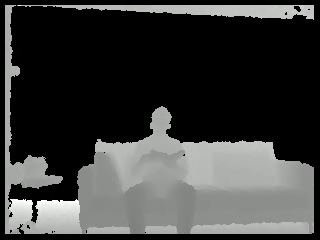
\includegraphics[width=0.45\textwidth]{ReadingBook.png}        
        }
    \hfill
    \subfloat[Drinking water]{
        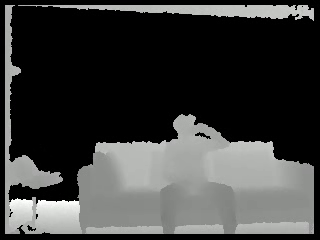
\includegraphics[width=0.45\textwidth]{DrinkingWater.png}        
        }
    \hfill
    \subfloat[Talking on a phone]{
        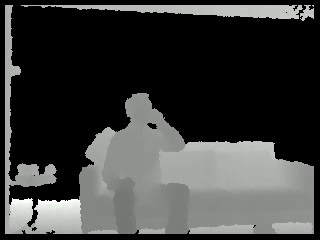
\includegraphics[width=0.45\textwidth]{TalkingOnAPhone.png}        
        }
    \hfill
    \subfloat[Playing game]{
        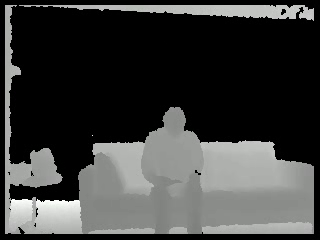
\includegraphics[width=0.45\textwidth]{PlayingGame.png}        
        }
    \hfill
    \subfloat[Writing on a paper]{
        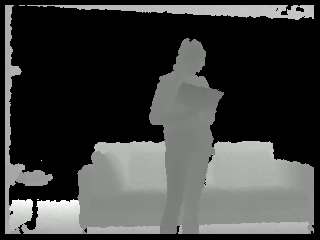
\includegraphics[width=0.45\textwidth]{WritingOnAPaper.png}        
        }
    \hfill
    \subfloat[Using a laptop]{
        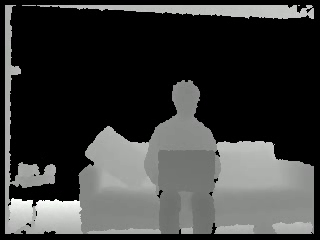
\includegraphics[width=0.45\textwidth]{UsingALaptop.png}        
        }
	\caption{\label{lbl:Figure_MSRDaily3D}Some sample actions on MSR Daily Activity 3D dataset.}
\end{figure*}

Although our method outperforms all the state-of-the-art methods, it is not our aim. It is important to note that why in condition of only using depth data, most of methods are failed. When considering failed samples, such as \textit{playing a game}, \textit{writing on a paper}, and \textit{using a laptop}, we found that most of them are confused with action \textit{still}. For \textit{playing a game}, main action focus on motion of fingers, it is very difficult to discriminate from depth noise. For \textit{writing on a paper} and \textit{using a laptop}, hand gestures are major actions to present motion information. But it is not fortunately, most of the movements are hidden by interactive objects (i.e. book, laptop). That is one reason to explain for the failure. The second one is performing similar movements with different objects, such as \textit{talking on the phone} and \textit{drinking water}. In these cases, objects are small and textureless, so, it is very difficult to identify them.  Therefore, if only depending on depth data, it it very challenging to recognize these actions exactly. Due to these reasons, in order to improve the performance of recognition systems in terms of interaction, adding more information related to interactive objects must be necessary.

\subsection{Early versus Late Fusion in Our Approach}

In terms of the fusion, \cite{snoek2005early} provided an interesting work. In this work, authors evaluated semantic concepts on two fusion schemes: early fusion and late fusion. They conducted experiments on the 2004 TRECVID benchmark dataset for visual modality and textual modality. Results indicated that the performance of the late fusion scheme is better than the performance of the early fusion scheme for most concepts. This evaluation are also applied for several multimodal-based analysis systems. However, the conclusion is reasonable or not for our approach, when considering each intensity representation as a modality. In order to answer this issue, we perform similar experiments on the late fusion scheme. In the experimental settings, we use the MBH descriptor to represent motion features and work on representation combinations: (front and side), (front and top) and (front, side and top). Experimental results in comparison between the early fusion scheme and the late fusion scheme are showed in figure \ref{lbl:Figure_EarlyLateFusion}.

\begin{figure}[h]
    \centering
    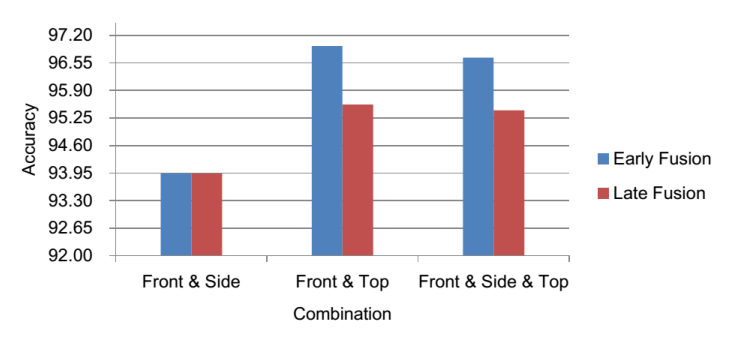
\includegraphics[width=0.47\textwidth]{Chart_EarlyLateFusion.eps}
	\caption{\label{lbl:Figure_EarlyLateFusion}Comparison of recognition accuracy on the early and late fusion schemes.}
\end{figure}

Figure \ref{lbl:Figure_EarlyLateFusion} indicates that both of the fusion schemes obtain significant improvements. However, the early fusion scheme gets better performances. Actually, we know that disadvantage of the early fusion approach is the difficulty to create a good feature representation, due to the semantic difference of modalities. To deal with this challenge, the late fusion approach is used to convert the representations into the same type of semantics (i.e. probability score). In our approach, due to the similarity of semantics between modalities (i.e. features to represent motion information), the performance of the early fusion approach will tend to be better than the one of the late fusion approach. Besides, the achieved results from combinations confirm again that selecting representations to merge motion information is not a trivial task.

\section{Conclusions}
\label{lbl:Conclusions}

We proposed the Pseudo-3D Trajectories, a 2D trajectory-based approach, for human action recognition using depth data in this work. We evaluated our approach by using the dense trajectory motion feature on the challenging datasets. More interestingly, our proposed trajectory-based approach only applied for one representation beats all the recent state-of-the-art approaches in terms of depth data. Besides, in order to deal with confused actions due to similar movements, compensating information from other representations is proposed. Therefore, the effectiveness of our approach on depth datasets like MSR is confirmed.

A trajectory-based approach with compensating information from separate representations shows promising results. This opens a general approach to leverage intensity-based techniques for depth data. This also suggests the importance of trajectory-based motion information on human action recognition using depth data. Therefore, exploiting depth-based motion trajectories can be beneficial for action recognition systems using depth cameras. This is also an interesting idea for our future work.

\section*{References}

\bibliographystyle{splncs}
\bibliography{JournalPaper_Ref}
\biboptions{sort&compress}

\end{document}